\chapter{Monoscopic Stitching Images}


%The fisheye camera images, the equirectangular projections and the corresponding cubemap images.

\begin{figure}[h]
	\begin{center}
		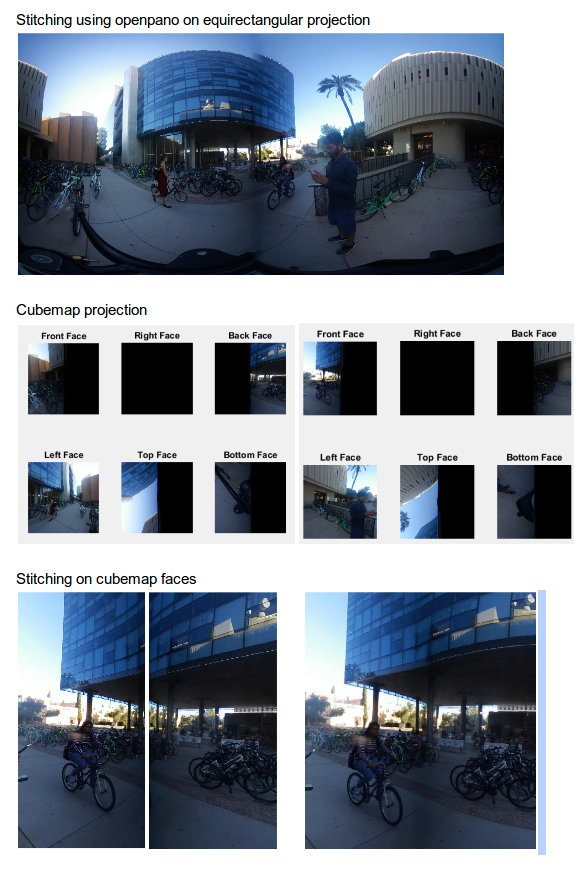
\includegraphics[width=0.7\textwidth]{/media/gunman/Data/thesis/ThesisLatex/data/images/CubeMapBasedStitching.png}
		\caption{Cubemap based Stitching} %, Path : /media/gunman/Data/fall-2017/research/mono360/equi2cubic}
		\label{ODS_Input_Output}
	\end{center}
	\vspace{-0.3in}
\end{figure} 

%Maximum Function For Extreme low power applications:
%Since the alignment techniques is not the final algorithm I may be going ahead with, I want to start with something even simpler, i.e a maximum function. We can imagine the core computation block as a black box, that can be changes as per the needs of the application. This becomes an interesting use case as the final camera could have multiple such black boxes which can be turned on and off based on application demand. For eg. If the camera is being used for CNNs, maximum function might be good enough. If it's going to be used for scene capture, then we can turn on an efficient stitching core instead of maximum function.





